\chapter{Determination of Tightening Coefficient of Threaded Joints}

\section{Nomenclature}
\begin{tabular}[t]{lp{6.5cm}}
	$ D_0 $ & outer diameter of the nut contacted with bolt, $ \unit{mm} $\\
	$ d  $ & nominal diameter of the bolt, $ \unit{mm} $\\
	$ d_0 $ & diameter of the bolt hole, $ \unit{mm} $\\
	$ d_2 $ & thread diameter, $ \unit{mm} $\\
	$ F_v $ & tightening force, $ \unit{N} $\\
	$ f $ & friction coefficient between nut and assemble part\\
\end{tabular}
\begin{tabular}[t]{lp{6.5cm}}
	$ K $ & tightening coefficient\\
	$ K_{exp} $ & tightening coefficient through experimentation\\
	$ K_{theo} $ & theoretical tightening coefficient\\
	$ p $ & thread height, $ \unit{mm} $\\
	$ T_r $ & force moment acting on thread,$ \unit{N\cdot m} $\\
	$ T_v $ & tightening moment, $ \unit{N\cdot m} $\\
	$ \delta_K $ & error between $ K_{exp} $ and $ K_{theo} $\\
	$ \gamma $ & back rake angle of thread, $ ^\circ $\\
	$ \rho' $ & the friction angle on the thread surface, $ ^\circ $
\end{tabular}

\section{Aim}
\begin{enumerate}
	\item Understand deeply the theory of screw coupling.
	\item Use the wrench to determine $ T_v $.
	\item Understand the principle and use load cell to measure the $ F_v $ on the	bolt;
	\item Determine $ K_{exp} = \dfrac{1000T_r}{F_vd} = \dfrac{1}{F_vd}\left[1000T_v-\dfrac{1}{2}\left(\dfrac{D_0+d_0}{2}\right)F_vf\right]$ and understand the relationship between $ T_v $ and $ F_v $, as well as the factors of assembling condition of the joint.
\end{enumerate}

\section{Technical rules on safety}
Students must comply with the technical rules on safety in the laboratory.

\section{Experimental report}

\subsection{Determine the parameters of threaded joint and measuring tools}
\begin{itemize}
	\item $ d_0=13.8\unit{(mm)} $
	\item $ D_0=18.8\unit{(mm)} $
	\item $ p=1.49\unit{(mm)} $
	\item $ d_2 = \dfrac{p}{\pi\tan\gamma} = 10.86\unit{(mm)}$
	\item $ \gamma=2.5^\circ $
	\item $ \rho'=10^\circ $
	\item $ f=0.25 $
\end{itemize}\clearpage
\subsection{Experimental results}
\begin{table}[h!t]
	\centering
	\rowcolors{5}{}{lightgray!20}
	\renewcommand{\arraystretch}{1.5}
	\begin{tabular}{crrr}
		\toprule
		&
		\multicolumn{3}{c}{Nominal diameter $d=12\unit{(mm)}$} \\ \cmidrule{2-4} 
		\multirow{-2}{*}{No.} &
		\multicolumn{1}{c}{$T_v$} &
		\multicolumn{1}{c}{$F_v$} &
		\multicolumn{1}{c}{$K_{exp}$} \\
		& \multicolumn{1}{c}{$ \unit{(N\cdot mm)} $} & \multicolumn{1}{c}{$ \unit{(N)} $} & \\
		\midrule
		1                   &  16.5                 &       2875            &  0.31\\
		2                  &     17.6              &       3243            & 0.28 \\
		3                   &      19.1             &         3938        & 0.23 \\
		4                   &   22.4                &      4872             & 0.21 \\
		5                   &   27.9                &        5229           &  0.27\\
		\multicolumn{3}{|c|}{\cellcolor[HTML]{C0C0C0}Average value} & 0.26 \\ \hline
	\end{tabular}
	\caption{The experimental results}
	\label{tab:my-table}
\end{table}
\begin{figure}
	\centering
	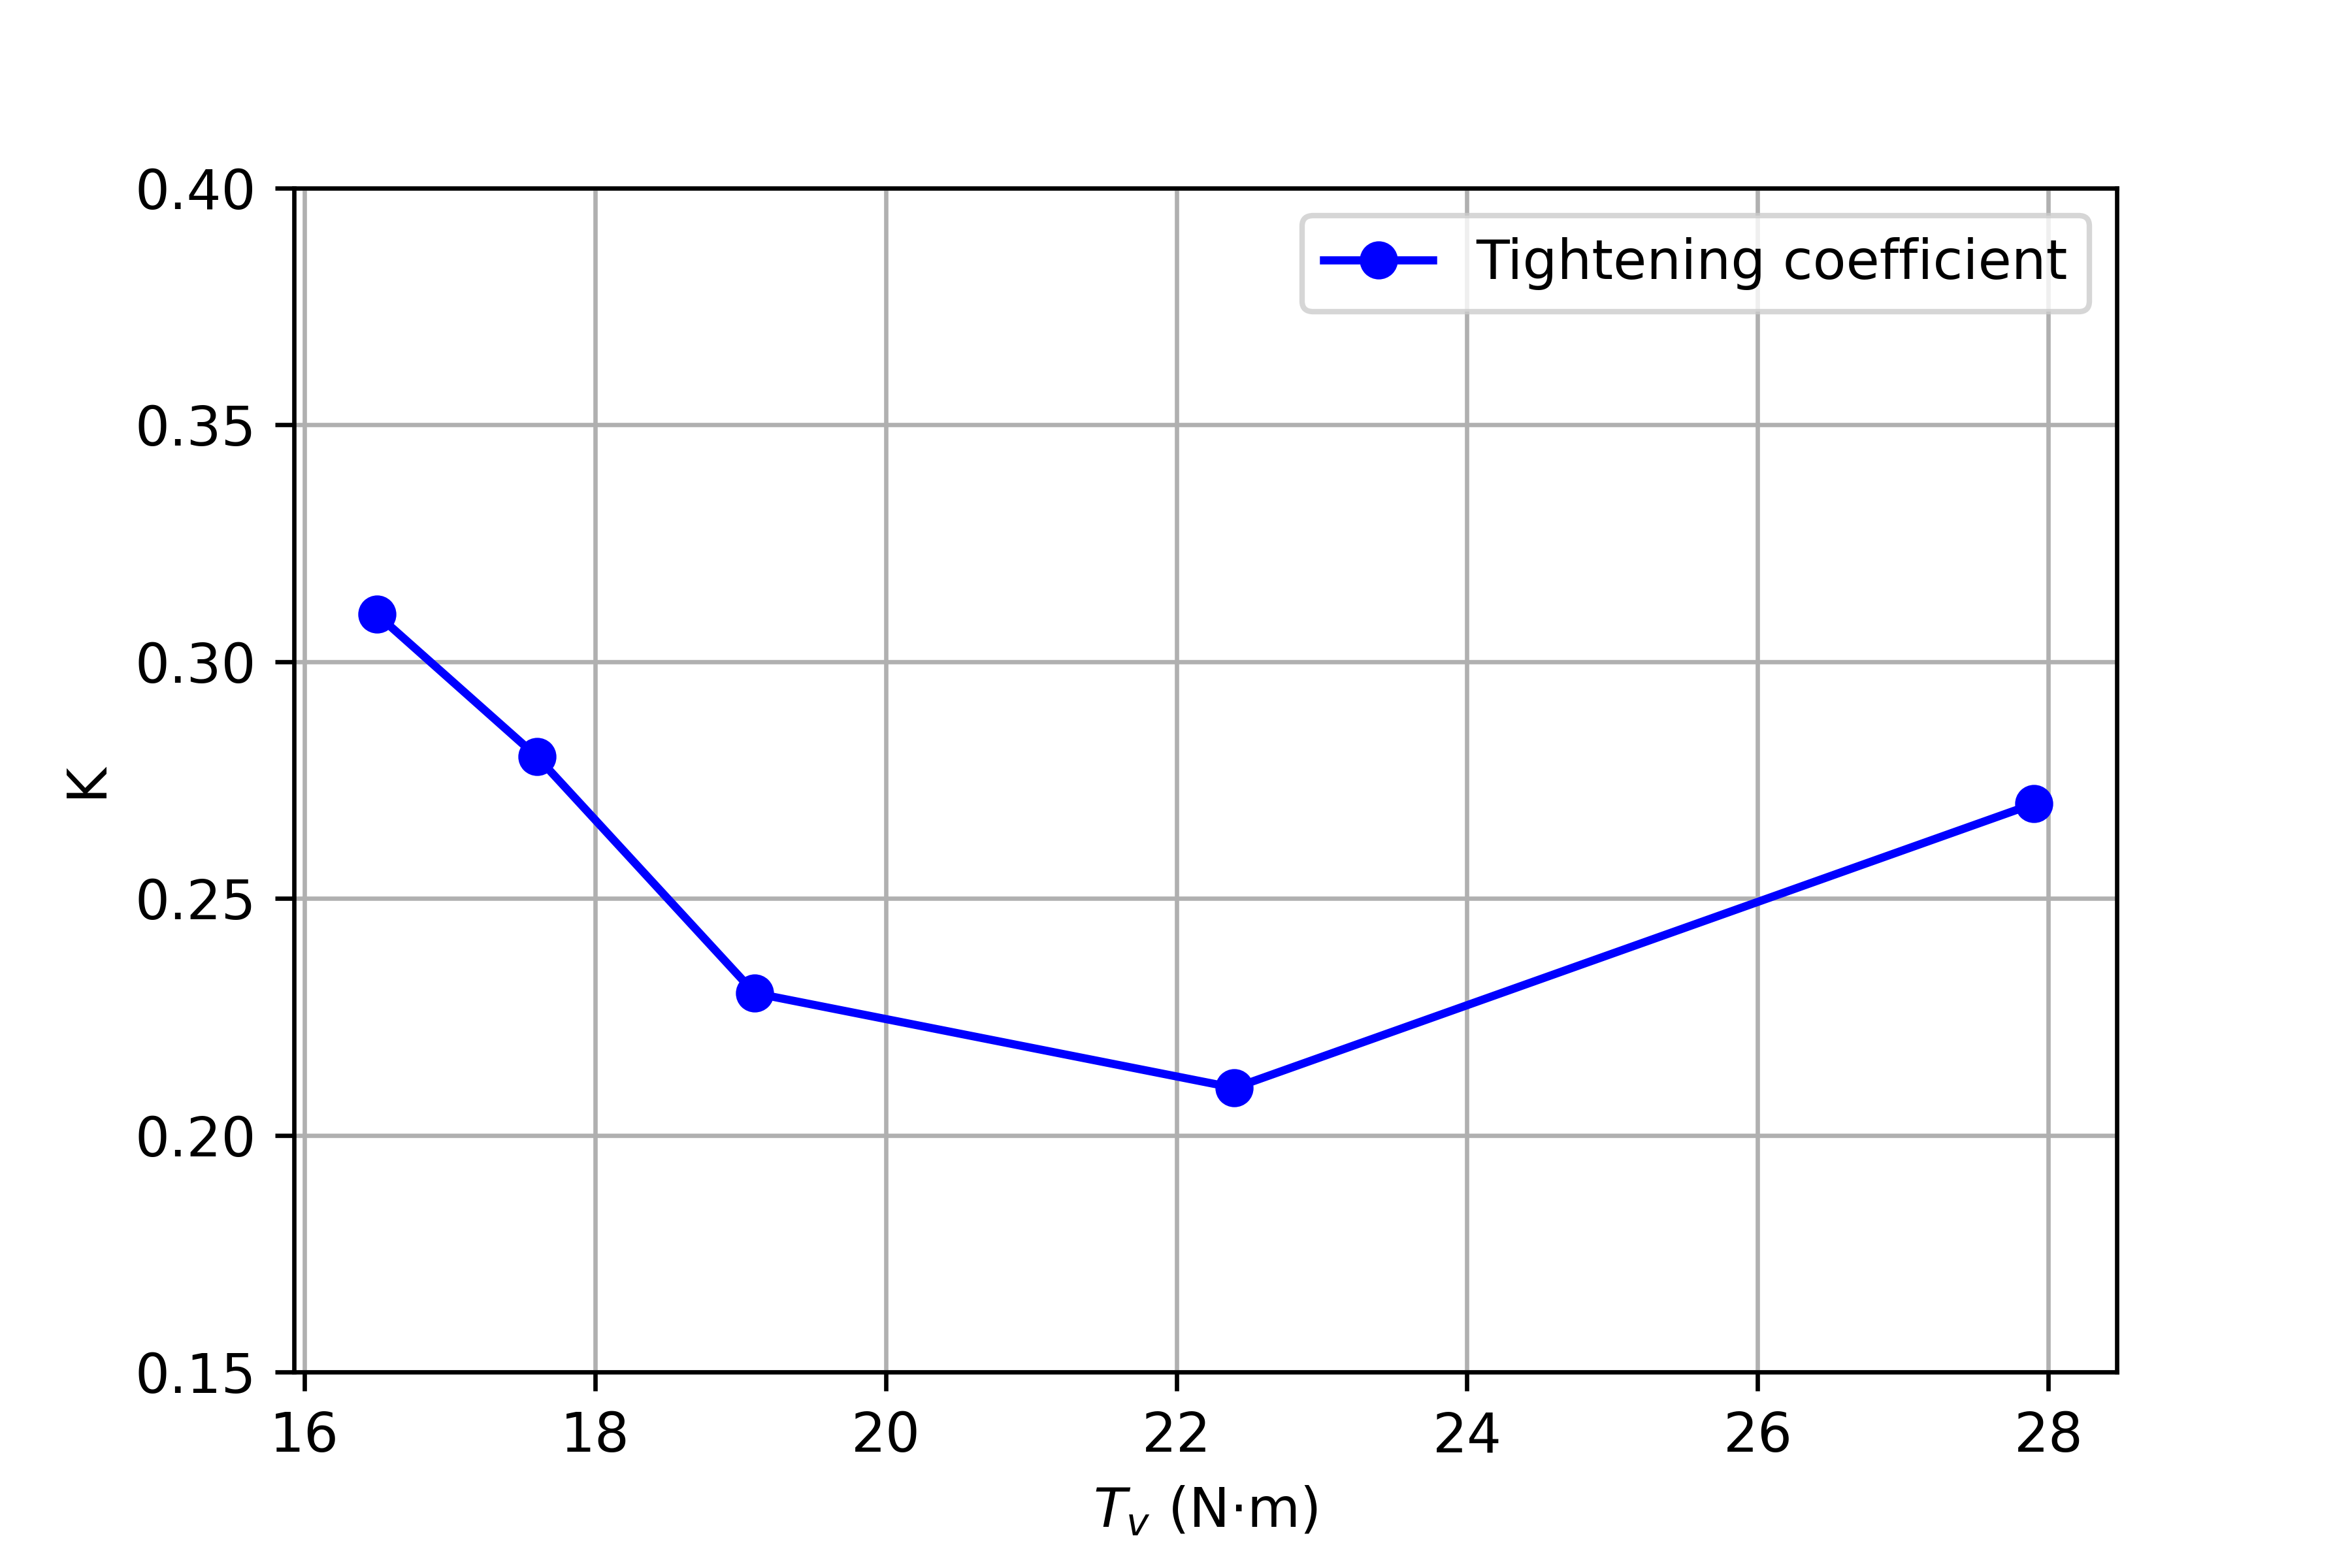
\includegraphics[width=150mm]{exp3.png}
	\caption{Relation between $ T_v $ and $ K_{exp} $ through experimentation}
	\label{tvk}
\end{figure}
\subsection{Compare theoretical results with experimental results}
The theoretical result $ K_{theo} $ is determined by the formula \[ K_{theo} = \dfrac{1000T_r}{F_vd} = 0.5\left(\dfrac{d_2}{d}\right)\left[\left(\dfrac{d_{0}+D_0}{2d_2}\right)f + \tan(\gamma+\rho')\right] = 0.27\]
Comparing $ K_{exp} $ and $ K_{theo} $ yields:
\[\delta_K = \dfrac{|K_{exp}-K_{theo}|}{K_{theo}} = 2.75\%\]

\section{Discussion and conclusions}
\begin{itemize}
	\item From the graph, the tightening coefficient and tightening moment have a linear relation.
	\item The error of $ K $ in the experiment compares to its theoretical counterpart is negligible ($ \pm 2.75\% $)
	\item Possible causes of error:
	\begin{itemize}
		\item The bolt is not tightened enough, reducing the value of measured tightening moment.
		\item Worn condition of the bolt affects the friction coefficient and thread angle.
		\item Error of the lab instrument (instability in displaying results), thus the measured values are only relative.
		\item  Rounding errors through calculations.
	\end{itemize}
\end{itemize}




\section{Review questions}
\begin{enumerate}
	\item \emph{Show the role and importance of finding $ F_v $ and $ T_v $ in reality.}\\
	Typically, an under torqued bolt will deform and be unable to provide as much clamping force as needed. An over torqued bolt will break.
	\item \emph{Explain the meaning of $ K $.}\\
	$ K $ is the synthesis of all the factors that affect the relationship between tightening moment and tightening force in reality, including friction, bending, elastic deformation of thread and many other factors that we may or may not already know. Therefore, it is difficult to determine accurately the tightening coefficient. It can only be determined relatively be experiments for each specific application. Typically, in a specific application, a value range of $ K $ is usually determined to predict the maximum and minimum values of the tightening force. Then, the initial tightening moment value is determined
	\item \emph{Explain the principles of ultrasonic operation and force measuring tool.}
	\begin{itemize}
		\item Ultrasonic sensors emit short, high-frequency sound pulses at regular intervals. These propagate in the air at the velocity of sound. If they strike an object, then they are reflected as echo signals to the sensor, which itself computes the distance to the target based on the timespan between emitting the signal and receiving the echo.
		\item As the distance to an object is determined by measuring the time of flight and not by the intensity of the sound, ultrasonic sensors are excellent at suppressing background interference.
		\item Virtually all materials which reflect sound can be detected, regardless of their color. Even transparent materials or thin foils represent no problem for an ultrasonic sensor.
	\end{itemize}	
	\item \emph{Determine $ K $ according to the theory of screw coupling.}\\
	The tightening factor $ K $ is the experimental coefficient. In comparison with the theory of screw coupling, we have the following relationship:
	\[ K_{theo} = \dfrac{1000T_r}{F_vd} = 0.5\left(\dfrac{d_2}{d}\right)\left[\left(\dfrac{d_{0}+D_0}{2d_2}\right)f + \tan(\gamma+\rho')\right] \]
	The parameters are defined in nomenclature.
	\item \emph{Compare $ K $ in cases of with and without lubrication to the joints. Then draw your conclusions.}\\
	In this experiment, three types of oil, grease, and solid film lubricants are investigated for their effect on the friction and torque-tension relationship in threaded fastener applications. The nut factor, the coefficients of thread and under-head friction were obtained from the experiments. The effect of the number of tightening and loosening cycles, the tightening speed and the lubricants on friction and nut factor were investigated. It was found that lubrication had a significant effect on the friction and the torque-tension relationship in threaded fasteners.\\
	Under the dry-and-cleaned condition, the nut factor for coarse threads is $ 0.181 $ and $ 0.1827 $ for fine threads during the first tightening. Comparing the three types of lubricants investigated, it can be seen that the solid film lubricants have the smallest thread friction and under-head bearing friction. Therefore, the same amount of input torque will generate a higher clamping force, which means lower nut factors. The greases and the oils have very similar friction behavior. However, for the low tightening speed case, the greases produce lower friction than the oils do.
\end{enumerate}